
\subsection{Fielding the survey}
The survey is fielded by Google Consumer Survey, under a simple contract with the purchaser. Respondents answer surveys in exchange for access to premium content, or (when using a custom app provided by Google) in exchange for credits in the Google Play Store, which can be used to purchase mobile apps, movies, etc. \citep{Google_Inc2016-fj}. Google suggests the following text when describing the data:
\begin{quotation}
	Google Surveys show questions across a network of premium online news, reference and entertainment sites, where it gets embedded directly into content, as well as through a mobile app, Google Opinion Rewards. On the web, users answer questions in exchange for access to that content, an alternative to subscribing or upgrading. The user's gender, age, and geographic location are inferred based on anonymous browsing history and IP address. On mobile, users answer questions in exchange for credits for books, music, and apps and users answer demographic questions when first downloading the app. Using this data, Google Surveys can automatically build a representative sample of thousands of respondents.
	{\footnotesize{Source: \url{https://support.google.com/360suite/surveys/answer/6324082}}}
\end{quotation}

\subsection{Creating the survey}
There is no influence by the researcher on the way the questionnaire is fielded. For instance, the displayed format, the type of website used to display the questionnaire, the visual format of the response (stars for Likert scales) cannot be changed. A researcher is not identified on the "INFO" screen that users can access from any screen (Figure~\ref{fig:info}). Potential respondents also have no way of seeing later questions.  \cite{doi:10.1093/pan/mpw016} note `` Given the  `survey wall' environment, it is essential that the surveys be short. ''  Researchers are also limited in the amount of information they can convey: only 175 characters are allowed for question text.

Other limitations include limitations on content. Google prohibits researchers from requesting personally and geographically identifying information \citep{Google_Inc2017-wi}. Sensitive demographics are subject to review by Google, and Google may choose to insert a disclaimer or permission screen. Sensitive opinions, such as ``abortions and sexual orientation'' \citep{Google_Inc2017-wi}, adult material, offensive questions,  may be censured by Google. 
\textbf{URLs are expressly forbidden.} 

\begin{figure}
	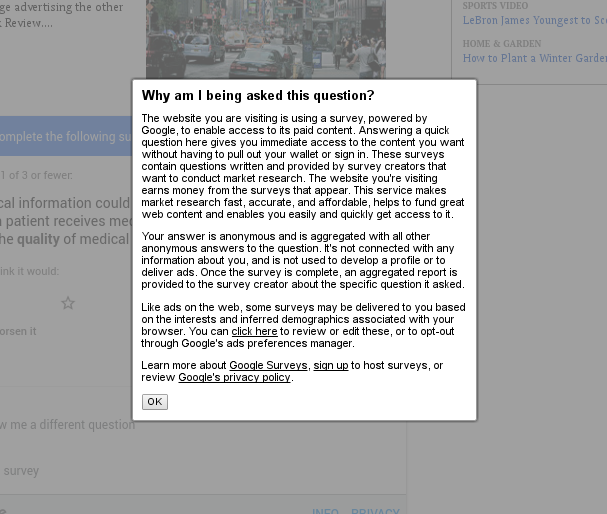
\includegraphics{Selection_365.png}
	\caption{\label{fig:info}Info screen}
\end{figure}



